\section{Алгоритмы, основанные на объединении критериев.}
1) «Скаляризация»: создание одного критерия оптимизации из нескольких
\begin{figure}[h]
Пример: взвешенная сумма: $F(x) = w_{1}f_{1}(x) + w_{2}f_{2}(x) + ...+ w_{k} f_{k} (x)$\\
Набор подфункций с рядом коэфициентов, который приводяк с скаляру, таким образом задача сводится к однокритериальной оптимизации.
\begin{center}
    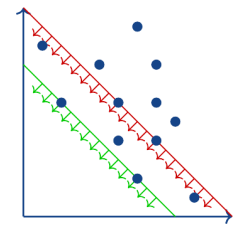
\includegraphics[width=0.35\linewidth]{images/Scalar.PNG}
    \caption{Пример скаляризации -взвешенная сумма}
    \label{fig:mpr}
\end{center}
\end{figure}
\begin{figure}[h]
Пример: подход Чебышева с весами (weighted Chebyshev):\\
$F(x) = max_{i} λ_{i}(f_{i}(x) − z_{i})$. То же самое, только идет максимизация заданного коэффициента
\begin{center}
    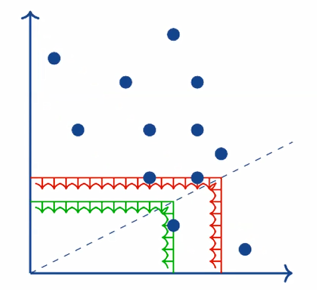
\includegraphics[width=0.35\linewidth]{images/Scalar_Chebyshev.PNG}
    \caption{Пример скаляризации - подход Чебышева с весами}
    \label{fig:mpr}
\end{center}
\end{figure}

Общие проблемы:\\
- Выбор параметров влияет на качество сведения задачи к однокритериальным (Например, подбор вектора весов в примере с взвешенной суммы)\\
- Изменение параметров влечет перезапуск оптимизатора, таким образом получаемые решения являются непрогнозируемыми из-за наличия данного внешнего фактора\\
- Не всегда все возможные оптимальные решения могут быть найдены (То есть мы имеем только локальные оптимальные решения)\\
С помощью взвешенной суммы нельзя найти решения не на выпуклой оболочке Парето-фронта\\
- Возможны нетривиальные проблемы со сходимостью\\
Частота получения новых решений в подходе Чебышева может скачкообразно и экспоненциально снижаться по мере приближения к фронту. Параметризация функции на рис. 2 ($f(x)$) зависит от итеративного процесса - на каждой итерации разное максимальное значение. Все это приводит к смешению - во-первых идёт процесс поиска глобального оптимума функции $f$, - с другой стороны идёт процесс скаляризации, не факт, что эти 2 процесса сойдутся, что приведёт алгоритм скаляризации (по Чебышеву) к генерации случайных чисел
